\section{Example}
\label{sec:example}

\begin{figure}[t]
\centering
\includegraphics[scale=0.8,clip]{figure/dataflow.eps}\vspace*{-3ex}
 \caption
{\label{fig:dataflow}API methods connected by inputs and
outputs}\vspace*{-3ex}
\end{figure}





Our approach accepts existing projects such as Lucene that have both
Java and C\# versions, and mines mapping relations of APIs. We refer
these existing projects as client code using the APIs of two
languages. First, our approach aligns classes and methods of the two
versions by using a matching algorithm based on similarities in the
names of classes and methods. Aligning client code based on names of
classes and methods is based on our observation of how existing
projects such as
rasp\footnote{\url{http://sourceforge.net/projects/r-asp/}} are
migrated from one language to another. We observed that while
migrating rasp project from Java to C\#, programmers first rename
source files from Java to C\# and systematically address the
compilation errors by replacing Java APIs with C\# APIs. During this
procedure, names of classes, methods, fields of classes, or local
variables in methods often remain the same between the two versions.
Therefore, we use name similarities for aligning client code of the
two versions. Second, our approach maps API classes of one language
with the other language by matching the names of fields of classes
and local variables of methods in the client code. Finally, our
approach maps API methods of one language with the other language.
Mapping API methods is challenging as one API method of one language
can be mapped to multiple API methods of the other language (as
shown in our preceding example).


We next use an example to illustrate challenges involved in
mining API mapping. Consider that a programmer needs to migrate
a Java code example (shown in Figure~\ref{fig:totranslation}) to C\# using a translation tool.
This code example accepts a \CodeIn{string} input that represents
name of a file or directory and returns a \CodeIn{boolean} value that
describes whether the file or directory exists. To achieve this functionality,
the code example declares a local variable, called \CodeIn{file},
of type \CodeIn{java.io.File} and calls the \CodeIn{exists} method.
We consider the local variable \CodeIn{file} as a receiver object for
the \CodeIn{exists} method.

To translate this code example into C\#, the translation
tool needs to know mapping relations of API classes. For example,
the translation tool needs to know the mapped API class for \CodeIn{java.io.File}
in C\# to translate the variable \CodeIn{file} to C\#. In addition, the translation tool needs
to know the mapped API methods of \CodeIn{exists}. Furthermore,
the translated code should be able to accept the same input
``\CodeIn{test}'' and produce the same output as the Java code example.

As APIs are often large in size, existing translation tools~\cite{}
(@Hao: Please add citations) often support only a subset of
mapping relations of used APIs. The reason for supporting only
a subset of mapping relations is that the mapping relations are written
manually in these translation tools. Therefore, the translation
tool cannot translate this Java code example, if the mapping relation
for the \CodeIn{java.io.File} does not exist. To address this issue,
a few translation other tools~\cite{} (@Hao, please add citations)
provide extensions for the programmer to write customized rules for translation.
However, to write customized rules, programmer needs to have
knowledge about both the languages. Furthermore, writing these
customized rules manually for all APIs is tedious and error-prone.

To address these preceding issues and to generate the rules for translation,
we propose a novel approach that automatically mines mapping
relations of APIs. Our approach uses existing projects such as
Lucene that have both Java and C\# versions, and mines
mapping relations of APIs. One would argue that given projects
such as Lucene with both Java and C\# versions, a programmer
can manually learn these mapping relations easily.
We next explain why it is not straightforward to learn these mapping relations of APIs
and how our approach addresses these challenges.

First, our approach aligns classes and methods of the two versions by using
a matching algorithm based on similarities in the names of classes
and methods between the two versions. For example, our approach aligns
\CodeIn{IndexFiles.java} with the \CodeIn{IndexFiles.cs}
(shown in Figure~\ref{fig:clientcode}) as the names of their classes and methods are similar.
Although it appears trivial, It is tedious task for the programmer to align
the classes manually as both versions can have large number of classes and methods.
For example, Lucene includes more than 1,000 classes.


\begin{figure}[t]
\begin{CodeOut}
\begin{alltt}
1  File file = \textbf{new} File("test");
2    \textbf{if}(file.exists())\{...\}
\end{alltt}
\end{CodeOut}\vspace*{-4ex}
\caption{\label{fig:totranslation} A code example for language
migration.}%\vspace*{-1ex}
\end{figure}
\begin{figure}[t]
\begin{CodeOut}\vspace*{-2ex}
\begin{alltt}
                  IndexFiles.java
3 public class IndexFiles \{
4   static final File INDEX_DIR = new File("index");
5   public static void main(String[] args) \{
      ...
6     if (INDEX_DIR.exists()) \{...\}
      ...
7       INDEX_DIR.delete();
    \}
  \}
                  IndexFiles.cs
8 class IndexFiles\{
9   internal static readonly System.IO.FileInfo INDEX_DIR
          = new System.IO.FileInfo("index");
10   public static void  Main(System.String[] args)\{
      ...
11     bool tmpBool;
12     if (System.IO.File.Exists(INDEX_DIR.FullName))
13       tmpBool = true;
14    else
15       tmpBool = System.IO.Directory
                         .Exists(INDEX_DIR.FullName);
      ...
    \}
 \}
\end{alltt}
\end{CodeOut}\vspace*{-4ex}
\caption{\label{fig:clientcode} Two versions (Java and C\#) of
client code.}\vspace*{-4ex}
\end{figure}

Even after the programmer successfully finds out the two aligned files, it is still
non-trivial to learn mapping relations of APIs. The programmer first
needs to map inputs of the three code snippets. In particular, by
comparing Line 1 with Line 4, the programmer knows that
\CodeIn{index} is the name for a file or a directory. Consequently,
the programmer analyzes how \CodeIn{index} in Line 4 (Java code) and
\CodeIn{index} in Line 9 (C\# code) are used in the two source files
for API mapping of interest so that boolean values are produced for
the functionality. To achieve so, the programmer may need to analyze
inputs and outputs of each API method. Figure~\ref{fig:dataflow}
shows API methods connected by inputs and outputs for the preceding
two files. In particular, a box denotes an API method, and an
ellipse denotes either an input or an output. The strategy of
analyzing inputs and outputs helps find out an API method like
\CodeIn{System.IO.Directory.Exists()}. This API method is called in
an assignment statement, whereas three other related API methods are
called in infix expressions of if-statements. If the programmer
relies on call-site structures only, the programmer can miss the API
method as its call-site structure is quite different. To match
outputs, the programmer must know the mapping relations of classes.
For this example, the programmer should know the mapping relation
between \CodeIn{boolean} in Java and \CodeIn{System.Boolean}. After
the inputs and outputs are mapped, the programmer needs to further
match functionalities. For this example, the \CodeIn{delete()}
branch of Figure~\ref{fig:dataflow} implements a different
functionality as indicated by its name, and thus this branch is not
mapped with other branches.

The programmer learns mapping relations of APIs from the preceding
analysis. However, the analysis is not accurate enough. In
particular, Figure~\ref{fig:dataflow} does not consider parameters
and fails to provide useful information if two API methods have
different parameter orders. For this example, as shown in Line 6,
the input of \CodeIn{java.io.File.exist()} is a variable, but the
inputs of \CodeIn{System.IO.Directory.Exist()} and
\CodeIn{System.IO.File.Exist()} are both their parameters as shown
in Line 12 and Line 15. The preceding analysis does not consider
parameters yet.
\begin{figure}[t]
\centering
\includegraphics[scale=0.65,clip]{figure/sample.eps}\vspace*{-3ex}
 \caption
{\label{fig:example}API mapping}\vspace*{-3ex}
\end{figure}

In this paper, we propose a novel approach that mines API mapping
automatically. Figure~\ref{fig:example} show the mined mapping
relation of APIs from the preceding two source files. In this
figure, a box denotes an API method. Here, our approach uses
\CodeIn{getFullName()} to denote the field access of
\CodeIn{FullName}. An ellipse denotes a parameter, a variable, or a
return value. Each ellipse is named as ``\emph{name:type}''. Here,
our approach uses ``variable'' for accesses of variables, ``null''
for return values, and parameter names for parameters.


The mined API mapping has matched inputs, outputs, and how inputs
and outputs are connected. Consequently, with the mined API mapping,
a translation tool can automatically translate the preceding code
snippet into C\# as follows:



In summary, for this example, we find that a programmer needs to
take tedious and error-prone efforts to find and to analyze source
files from two versions of a project for API mapping. We next
present our approach to mine API mapping automatically.


%Based on the mapping relations, a translation tool can migrate the
%preceding code snippet automatically. To learn the mapping
%relations,
%
%%\begin{figure}[t]
%%\centering
%%\includegraphics[scale=0.86,clip]{figure/openfile.eps}\vspace*{-1.5ex}
%% \caption
%%{\label{fig:openfile}Aligned client code}\vspace*{-2ex}
%%\end{figure}
%
%In this section, we illustrate the main steps of our approach to
%mine the API mapping in Java for \CodeIn{System.IO.Directory.
%Exists()} in C\# from the HypoLog
%project\footnote{\url{http://sourceforge.net/projects/twlog/}}.
%
%The first step of our approach is to align classes and methods of
%client code by names. This step finds class pairs and method pairs
%that implement similar functionalities, and each pair may use
%API mapping since it implements a similar functionality. Our
%approach chooses names to align classes and methods because these
%classes and methods are from the same project. In this example, our
%approach aligns the two methods as shown in
%Figure~\ref{fig:openfile} because the two method have similar names
%and their declaring classes also have similar names (see
%Section~\ref{sec:approach:alignclientcode} for details).
%
%The second step of our approach is to mine mapping relations of API
%classes based on the names of corresponding fields, parameters,
%returned types, and local variables. This step also relies on names
%for the same consideration of the first step. For example, our
%approach maps the two parameters with the same name as shown by the
%red arrow of Figure~\ref{fig:openfile}. From the types of the two
%parameters, our approach mines the mapping relation between two API
%classes: \CodeIn{System.String} $\leftrightarrow$
%\CodeIn{java.lang.String} (see
%Section~\ref{sec:approach:mappingtypes} for details).
%
%
%The final step of our approach is to mine mapping relations of API
%methods. Besides the factors listed in
%Section~\ref{sec:introduction}, another factor is that API calls in
%client code are often not carefully aligned. To deal with those
%challenges, our approach first builds an API Transformation Graph
%(ATG) for each method. After that, our approach compares built
%graphs to mine mapping relations of API methods (see
%Section~\ref{sec:approach:mappingtypes} and
%Figure~\ref{fig:approach1} for details). Figure~\ref{fig:example}
%shows the mined mapping relation between
%\CodeIn{System.IO.Directory.Exists()} and its API mapping in
%Java.
